% resume.tex
%
% (c) 2002 Matthew Boedicker <mboedick@mboedick.org> (original author) http://mboedick.org
% (c) 2003-2007 David J. Grant <davidgrant-at-gmail.com> http://www.davidgrant.ca
%
% This work is licensed under the Creative Commons Attribution-ShareAlike 3.0 Unported License. To view a copy of this license, visit http://creativecommons.org/licenses/by-sa/3.0/ or send a letter to Creative Commons, 171 Second Street, Suite 300, San Francisco, California, 94105, USA.
\documentclass[letterpaper,11pt]{article}
%-----------------------------------------------------------

\immediate\write18{git rev-parse --short HEAD > version.info }

%Margin setup

\setlength{\voffset}{0.1in}
\setlength{\paperwidth}{8.5in}
\setlength{\paperheight}{11in}
\setlength{\headheight}{0in}
\setlength{\headsep}{0in}
\setlength{\textheight}{11in}
\setlength{\textheight}{9.5in}
\setlength{\topmargin}{-0.25in}
\setlength{\textwidth}{7in}
\setlength{\topskip}{0in}
\setlength{\oddsidemargin}{-0.25in}
\setlength{\evensidemargin}{-0.25in}
%-----------------------------------------------------------
%\usepackage{fullpage}
\usepackage{shading}
\usepackage{hyperref}
\usepackage{fancyhdr}
\usepackage{graphicx}
\usepackage{xcolor}
%\textheight=9.0in
\pagestyle{fancy}

\fancyhead{}
\fancyhead[RE,LO]{\textbf{\Large{Dominique Dierickx}}}
\fancyhead[LE,RO]{\href{https://www.dominiek.eu}{https://www.dominiek.eu}}
\fancyfoot{}
\fancyfoot[LE,LO]{\textcolor{gray}{\input{version.info}}}
\fancyfoot[RO, RE]{\thepage}

\raggedbottom
\raggedright
\setlength{\tabcolsep}{0in}

%-----------------------------------------------------------
%Custom commands
\newcommand{\resitem}[1]{\item #1 \vspace{-2pt}}
\newcommand{\resheading}[1]{{\large \parashade[.9]{sharpcorners}{\textbf{#1 \vphantom{p\^{E}}}}}}
\newcommand{\ressubheading}[4]{
	\begin{tabular*}{6.5in}{l@{\extracolsep{\fill}}r}
		\textbf{#1} & #2 \\
		\textit{#3} & \textit{#4} \\
	\end{tabular*}\vspace{-6pt}}
\newcommand{\ressubheadingsimple}[1]{
	\textbf{#1} \\
	\vspace{-6pt}}
%-----------------------------------------------------------


\begin{document}
	
	\begin{tabular*}{7in}{l@{\extracolsep{\fill}}r}
		
	\end{tabular*}
	
	\vspace{0.1in}
	\vspace{0.1in}
	\resheading{Facts}
	\centering
	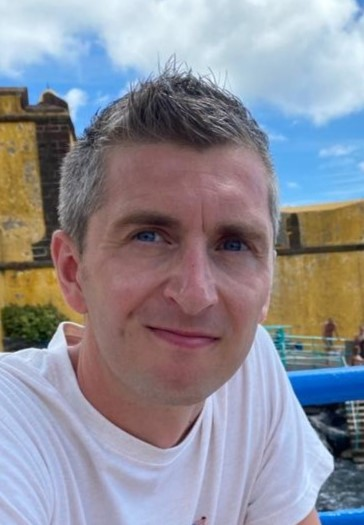
\includegraphics[width=0.5\textwidth]{me.jpg}
	\label{fig:my_label}
	
	\begingroup
	\leftskip3em
	
	\begin{tabular*}{0.75\textwidth}{@{\extracolsep{\fill}} l l }
		Gender & Male \\
		E-mail address & \href{mailto:d.dierickx@gmail.com}{d.dierickx@gmail.com} \\
		Nationality & Belgian \\
		Mother tongue & Dutch  \\
	\end{tabular*}
	\\
	
	\endgroup

	\hfill \break
\resheading{Work Experience}

\begin{itemize}
	
	\item
	\ressubheading{Showpad}{Ghent}{Principal Software Engineer}{November 2019 - now()}
	\begin{itemize}
		\resitem{Maintenance, bugfixing, evolution and monitoring of the SaaS-platform.}
		\resitem{Technical coordination and communication across teams.}
	\end{itemize}
	
	\item
	\ressubheading{Cegeka Belgium NV}{Ghent}{Application Architect}{January 2019 - November 2019}
	\begin{itemize}
		\resitem{Discuss requirements and feasibility with customers.}		
		\resitem{Project estimation and cost calculation.}	
		\resitem{Implementing the designed architectures together with the teams.}
		\resitem{Mentoring}
	\end{itemize}
	
	\item
	\ressubheading{TomTom Belgium NV}{Ghent}{Senior Software Architect in the Maps Unit}{January 2017 - January 2019}
	\begin{itemize}
		\resitem{Discuss requirements and feasibility with internal and external customers.}		
		\resitem{Designing and evolving our software architecture.}	
		\resitem{Implementing the designed architectures together with the teams.}
		\resitem{Technical coordination and communication across teams.}
	\end{itemize}
	
	\item
	\ressubheading{TomTom Belgium NV}{Ghent}{Expert Software Engineer in the Maps Unit}{January 2012 - January 2017}
	\begin{itemize}
		\resitem{Development of scalable map creation \& conversion tools.}
		\resitem{Design \& Development of B2B map delivery systems.}
		\resitem{Deployment and production support.}
	\end{itemize}
	
	\item
	\ressubheading{TomTom Belgium NV}{Ghent}{Software Engineer in the Research \& Development Unit}{February 2011 - December 2011}
	\begin{itemize}
		\resitem{Technical analysis and implementation of EU funded projects.}
		\resitem{Internal research projects.}
	\end{itemize}
	
	\item 
	\ressubheading{Adenti NV}{Zottegem}{Software developer}{September 2009 - January 2011}
	\begin{itemize}
		\resitem{Development of a web-based tracking and tracing system.}
		\resitem{Extending and improving the inhouse rapid application development framework.}
		\resitem{E-commerce web development.}
	\end{itemize}
	
\end{itemize}
	
		\hfill \break
	\resheading{Education}
	\begin{itemize}
		
		\item
		\ressubheading{Vrije Universiteit Brussel}{Brussels}{Master in Applied Computer Science}{2007-2009}
		\begin{itemize}
			\resitem{Graduated with great honor}
			\resitem{Master's thesis: ``Supporting smart entity behavior across virtual environment platforms''}
		\end{itemize}
		
		\item
		\ressubheading{Koninklijk Technisch Atheneum Geraardsbergen}{Geraardsbergen}{Latin - Mathematics}{1998 - 2004}
		\\
		
		\item
		\ressubheading{Hogeschool Gent}{Ghent}{Bachelor in Applied Computer Science}{2004-2007}
		\begin{itemize}
			\resitem{Graduated with honor}
			\resitem{Internship at Ordina Belgium}
		\end{itemize}
		
	\end{itemize}
	
	\resheading{Skills Summary}
	
	\begin{description}
		\item[Languages:]
		Java, Kotlin, Python, Javascript, Typescript, Shell scripting
		\item[Frameworks \& tools:]
		Spring (Boot), Micronaut, IntelliJ, VSCode, JUnit, Testcontainers, Docker
		\item[Databases:]
		PostgreSQL, MySQL, SQLite, ElasticSearch
		\item[Platforms:]
		Amazon Web Services, Kubernetes
		\item[Principles:]
		API design \& documentation, event-driven, software architecture, DDD, CI/CD, testing, devops.
		\item[Interests:]
		Artificial intelligence, cybersecurity, Geospatial Information Systems (GIS), large-scale data solutions, algorithms
    \end{description}
	
	
	\resheading{In a nutshell...}
	I am a driven, social person, interested in various fields and developments in computer science. My strongest points are my technical expertise, my eagerness to learn new things and my social skills. I have gained relevant experience through personal as well as professional projects and it is fair to say that software development is more of a passion than a profession in my life. In my spare time, I enjoy running, reading, experimenting with new technology and spending time with my wife and our two boys.
		\vspace{0.1in}

	\resheading{I am looking for}
    A position where I can make a difference and get things done. Working closely together with all stakeholders for the best possible outcome. In an environment that nurtures engineering culture and knowledge sharing.
	
\end{document}